\documentclass[a4paper, 12pt]{article}
\usepackage{graphicx}
\usepackage[usenames, dvipsnames]{color}
\graphicspath{ {./figure/} }
\begin{document}

    \title{Linux Tutorial for the Uninitiated}
    \maketitle

    \section{The "boot" has non space remaining}

    If you are out of storage space, you can $\bf Safely Removing Old Kernels.$ The problems can be fixed quickly and 
    easily from the shell. Besides, \emph{apt-get} can not remove a package due to broken dependency, while the \emph{dpkg} can.

    \begin{figure}[h]
        \caption{The Worning: The volume "boot" has only XX disk space remaining.}
        \centering
        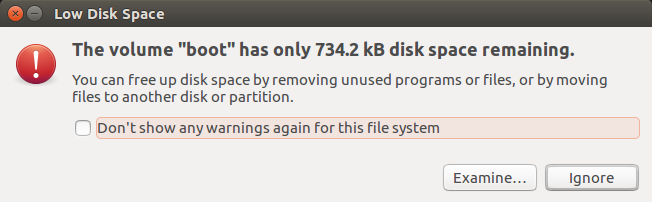
\includegraphics[width=0.8\textwidth]{fig1.png}
    \end{figure}


    \$ uname -r 
      
    \emph{This command identifies the currently-running kernel
    4.2.0-21-generic                   
    This is the current kernel. DO NOT REMOVE it!}

    \$ dpkg -l \text{\textbar} tail -n +6 \text{\textbar} grep -E 'linux-image-[0-9]+' \text{\textbar} grep -Fv \$(uname -r)

    \emph{This command lists all the kernels excluding the booted. kernel in the package database, and their status.}

    rc  linux-image-4.2.0-14-generic

    \emph{The oldest kernel in the database. Status 'rc' means it's already been removed}

    ii  linux-image-4.2.0-15-generic

    \emph{The oldest installed kernel. Eligible for removal. Status 'ii' means Installed.}

    iU  linux-image-4.2.0-22-generic

    \emph{DO NOT REMOVE. Status 'iU' means it's not installed, but queued for install in apt. This is the package we want apt to install. Purge the oldest kernel package using dpkg instead of apt.}

    \$ sudo dpkg --purge linux-image-4.2.0-15-generic

    \emph{If the previous command fails, some installed pack, depends on the kernel. The output of dpkg tells the name of the package. Purge it first.
    Also purge the respective header package.}

    \$ sudo dpkg --purge linux-headers-4.2.0-15-generic

    Try also purging the common header package.

    \$ sudo dpkg --purge linux-headers-4.2.0-15

    Do not worry, if the previous command fails.

    \$ sudo apt-get -f install 

    Try to fix the broken dependency.

    \section{Install the Jupyter}
    Before you start to set up the installing, you have to unstall ipython (including notebook).

    \textbf{Step 1. Installing Python 2.7 and pip}\\
    ......\\
    \$ python --version\\
    It will echo:\\
    \textit{Python 2.7.11+}\\
    \$ pip --version\\
    \textit{pip 8.1.1 from....}

    \textbf{Step 2.Install Ipython and Jupyter Notebook}\\
    First install Ipython:\\
    \begin{verbatim}
        $ sudo apt-get -y install ipython ipython-notebook
        $ sudo -H pip install jupyter
    \end{verbatim}

    \textbf{Step 3. Running Jupyter Notebook}\\
    \$ jupyter notebook

    If it wont work and response with \textbf{\textcolor{red}{"Native kernel (python2) not available"}} when you launch the jupyter notebook,
    you would better apply  \textbf{\textit{sudo -H pip install ipykernel}} to add non-native python kernel.

    %%%%%%%% new section

    \section{The difference between \textit{apt-get purge} and \textit{apt-get remove}?}
    As the \textbf{man apt-get} page says:\\
    \textbf{\textcolor{blue}{remove}}: Packages installed are removed (Dose \textbf{NOT} include cofiguration files)\\
    \textbf{\textcolor{blue}{purge}}: Purge is idential to \textcolor{blue}{remove} expect
    that packages are removed amd purged. Purge means that any configuration files are deleted too.
    This is of course does not apply to packages which hold configuration files inside the user's home 
    folder (eg: /home/tongust/), this files will not be touched.\\
    
    \section{How to add the \textbf{PATH} and environment}
    \textbf{With respect to JDK. }\\
    \begin{verbatim}
        1. Install JDK
        2. For "JAVA_HOME" (Environment Variable), type as follow:
        $ export JAVA_HOME=/home/tongust/jdk1.8.0_121
        $ export PATH=$PATH:/home/tongust/jdk1.8.0.0_121/bin
    \end{verbatim}

    \section{Install Caffe on ubuntu 16.04}
    Ref: https://huangying-zhan.github.io/2016/09/09/GPU-and-Caffe-installation-in-Ubuntu.html#Caffe\%20installation\\
    And: http://askubuntu.com/questions/799184/how-can-i-install-cuda-on-ubuntu-16-04\\
    Four step:\\
    1. Download CUDA\\
    3. Remove any other installtion ( \textit{sudo apt-get purge nvidia-cuda*}. If you want to install the driver in the .run, the \textit{sudo apt-get purge nvidia*} )\\
    ~~~~3.1 If you want install the display drivers, logout from your GUI, and get to tty1 (\textit{Ctrl + Alt + F1/F~6}, use \textit{Ctrl + Alt + F7 to back GUI})\\
    ~~~~3.2 Stop lightdm: \textit{sudo service lightdm stop}\\
    4. \textit{sudo sh cuda\_.run --override}. Make sure you say y for the symbolic link.\\
    ~~~~4.1 Start lightdm again: \textit{sudo service lightdm start}\\
    5. Export CUDA environment\\
    \begin{verbatim}
	echo "# Add CUDA bin & library paths:" >> ~/.bashrc
	echo "export PATH=/usr/local/cuda/bin:$PATH" >> ~/.bashrc
	echo "export LD\_LIBRARY\_PATH\=/usr/local/cuda/lib:\$LD\_LIBRARY\_PATH" >> ~/.bashrc
	source ~/.bashrc
    \end{verbatim}
    6. Install dependencies\\
    \begin{verbatim}
    #Install general dependencies

    sudo apt-get install libprotobuf-dev libleveldb-dev libsnappy-dev libopencv-dev libhdf5-serial-dev protobuf-compiler

    sudo apt-get install libboost-all-dev
    # If you get " E: Failed to fetch http://cn.archive.ubuntu.com/ubuntu
    /pool/universe/b/boost1.58/libboost-graph1.58-dev_1.58.0+
    dfsg-5ubuntu3.1_amd64.deb  Hash Sum mismatch"
    Try sudo  apt-get update.

    # Install ATLAS

    sudo apt-get install libatlas-base-dev
    # Install remaining dependencies
    sudo apt-get install libgflags-dev libgoogle-glog-dev liblmdb-dev
    Other issue: compilation failure due to "hdf5.h" 
    add the Makefile.config
    INCLUDE_DIRS := $(PYTHON_INCLUDE) /usr/local/include /usr/include/hdf5/serial/
    LIBRARY_DIRS := $(PYTHON_LIB) /usr/local/lib /usr/lib /usr/lib/x86_64-linux-gnu/hdf5/serial/
    see: https://github.com/BVLC/caffe/issues/2690
    \end{verbatim}
    https://github.com/BVLC/caffe/wiki/Ubuntu-16.04-or-15.10-Installation-Guide

    \section{Run a script at start up}
	Alternative #3: Add an init script (obsolete)

	Create a new script in /etc/init.d/myscript.

	vi /etc/init.d/myscript
	(Obviously it doesn't have to be called "myscript".) In this script, do whatever you want to do. Perhaps just run the script you mentioned.

	#!/bin/sh
	/path/to/my/script.sh
	Make it executable.

	chmod ugo+x /etc/init.d/myscript
	Configure the init system to run this script at startup.

	update-rc.d myscript defaults



    
\end{document}
